\section{Dynamic Systems}

\begin{center}
    Notes from \textbf{MECHENG 360: Modeling, Analysis, and Control of Dynamic Systems}

    Taken at University of Michigan, Winter 2026
\end{center}

\subsection{Classification of Systems}

A \textbf{signal} is a measurable quantity which may vary with time. Examples of signals may include force, velocity, temperature, position, or any other quantity which may vary with time. A \textbf{system} is a collection of components which act, typically in response to an input signal, and which produce an output signal.

Every system includes a \textit{compensator}, which is also called a \textit{controller}; a physical system, or \textit{plant}; a \textit{sensor}; and an \textit{actuator} which produces the output signal. A \textbf{block diagram} is a graphical tool used to visualize the interaction between signals and systems, with signals represented as arrows into or out of boxes which represent the system components. A common general structure for control systems is given in the block diagram below; note that the actuator is combined with the plant in this diagram, but in general these may be different blocks:
\begin{center}
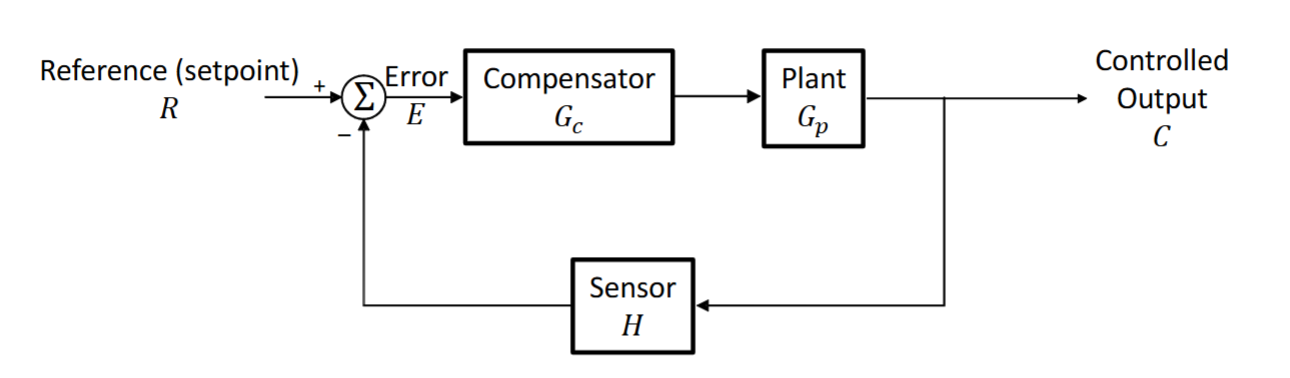
\includegraphics[width=0.85\linewidth]{Images/controls_standardsystem.png}
\end{center}
Note that these block processes execute simultaneously and constantly during operation. While some real-world systems operate with delay, i.e. microcontrollers which take inputs at fixed time intervals, it is generally a reasonable simplifying assumption that these systems operate continuously rather than discretely.

There are several ways to classify systems. The methods and mathematical techniques necessary for modeling a system depends on their classification.

A system is called \textbf{static} if present values of the system outputs depend only on the present values of the system inputs. As a consequence, static systems are describable with algebraic equations. In contrast, a system is called \textbf{dynamic} if the present value of the output signal depends on past values (and potentially present values as well) of the input signal. As a consequence, dynamic systems require differential equations to describe their behavior.

A \textit{system} is \textbf{time-invariant} if it has the property that delaying the input signal $u(t)$ by any constant $\tau$ results in an output signal $y(t)$ which is also delayed by $\tau$. An alternative classification is that a system is time-invariant if $t$ only appears as an argument of $u=u(t)$ and/or $y=y(t)$; for example, the differential equation $\dot y(t) + 2y(t) = u(t)$ is time-invariant, but $\dot y + 2ty = u(t)$ is time-variant. Note that, after substituting an explicit time-dependent expression for $u$, it is not generally possible to determine if a process is time-variant or time-invariant.

A static system $f(y)=g(u)$ is \textit{linear} if and only if we have the familiar conditions: \[f(c_1y_1 + c_2y_2) = c_1f(y_1) + c_2f(u_2)\hspace{0.2in} \forall c_1,c_2,y_1,y_2\in\mathbb{R}\]
\[g(c_1u_1 + c_2u_2) = c_1g(u_1) + c_2g(u_2)\hspace{0.2in} \forall c_1,c_2,u_1,u_2\in\mathbb{R}\] This definition readily extends to dynamic systems; in particular, a dynamic system is linear if and only if it can be written in the following form without constant offsets and with every term linear in its non-time arguments: \[f_n(y^{(n)},t) + \cdots + f_1(y',t) + f_0(y,t) = g_m(u^{(m)},t) + \cdots + g_1(u',t) + g_0(u,t)\]

\subsection{Mathematical Modeling of System Processes}

%%% Models for mathematical expressions for system processes:
%%% Differential equations models
%%% Transfer Functions
%%% State Space Models

Mathematical modeling of dynamic systems involves differential equations. The \textit{order}, or \textit{degree} of a differential equation is given by the highest derivative of the output variable. If the degree of the output variable is strictly greater than the degree of the input variable, then the system is called \textit{strictly causal}, meaning the present output depends \textit{only} on past inputs. When the degree of the output variable equals the degree of the input variable, the system is \textit{causal} but not strictly, meaning present output depends on the present input. A system is \textit{non-causal} if the degree of the output variables is strictly less than the degree of the input variables, meaning present output depends only on future inputs.

A strictly causal system does \textit{not} experience an immediate jump in outputs for a jump in inputs; a system which is causal but not strictly causal \textit{does} experience an immediate jump in outputs for a jump in inputs. Non-causal systems do not exist in the real world.

The systems studied are generally represented by linear, time-invariant ordinary differential equations. Analysis of dynamic systems then involves either solving for the outputs $y(t)$ explicitly given an input signal $u(t)$ and initial conditions, or it involves determining properties or features of $y(t)$ which must hold regardless of the properties of $u(t)$, i.e. ensuring that output signals respond quickly, avoid blow-up, and minimize oscillations when relevant.

% separation of variables
% method of undetermined coefficients
% laplace transforms

Consider a differential equation of the form \[y^{(n)} + a_{n-1}y^{(n-1)}+\cdots+a_1y' + a_0y = b_mu^{(m)} + \cdots + b_1 u' + b_0u\] There are two methods to solve differential equations of this form. These methods are the \textbf{method of undetermined coefficients}, and the method of \textbf{Laplace transforms}.

\begin{framed}
\textbf{Method of Undetermined Coefficients}. From differential equations theory, the solution $y(t)$ is given by the linear combination \[y(t) = y_h(t) + y_p(t)\] where the homogeneous component is the solution to the differential equation with $b_0=b_1=\cdots=b_m=0$, and is of the form \[y_h(t) = c_1 e^{\lambda_1 t} + \cdots + c_n e^{\lambda_n t}\] where Euler's identity relates the complex exponential solutions to real solutions: \[e^{j\theta} = \cos\theta + j\sin\theta\] Note the notational change that $j^2=-1$. The particular solution, $y_p(t)$, is of the form:

\begin{center}
    \begin{tabular}{c|c}
        $u(t)$ & $y_p(t)$ \\
        \hline\hline
        $k$ & $k_0$ \\
        $\sin(\omega t)$ & $k_0\sin(\omega t) + k_1\cos(\omega t)$\\
        $kt$ & $k_0 t + k_1$\\
        \end{tabular}
\end{center}

In a linear system, the homogeneous solution describes the transient behavior of the solution, and the particular solution describes the long-term behavior.
\end{framed}

\textbf{Example}. Consider the differential equation $\dot x +ax = b$. Since $x_h(t)$ is of the form $x_h(t) = ce^{\lambda t}$, the derivative is given by $\dot x_h(t) = c\lambda e^{\lambda t}$. Substituting this into the \textit{homogeneous} form of the differential equation, with $b=0$, gives: \begin{eqnarray*}
    c\lambda e^{\lambda t} + ace^{\lambda t} &=& 0\\
    \implies ce^{\lambda t} (\lambda + a) &=& 0\\
    \implies \lambda + a &=& 0\\
    &\implies& \boxed{\lambda = -a}
\end{eqnarray*} Thus, $x_h(t) = ce^{-at}$ for some value of $c$.

The non-homogeneous term is constant, so the particular solution is of the form $x_p(t)= k_0$. Therefore, $\dot x_p(t)=0$, and substitution into the differential equation gives: \[ak_0 = b \implies k_0 = \frac{b}{a}\] Therefore, the solution is given by \[x(t) = ce^{-at} + \frac{b}{a}\] Solving for $c$ with initial condition $x(0)=x_0$ gives: \begin{eqnarray*}
    x(0) &=& c + \frac{b}{a}\\
    \implies c &=& x(0)-\frac{b}{a}\\
    &\implies& \boxed{x(t) = \left(x(0) - \frac{b}{a}\right) e^{-at} + \frac{b}{a}}
\end{eqnarray*} The \textit{transient response} is given by the exponential component of this solution, and the \textit{forced response} is given by the constant $b/a$.

First and second order systems have a \textbf{time constant}, which is a measure of how fast the system decays. In a first order system with transient solution of the form $y_h\propto e^{-at}$, the time constant is given by \[\tau = \frac{1}{a}\] which is the time necessary for approximately $63\%$ solution decay. If $a<0$, the solution tends towards $\pm\infty$ instead, and a measure of the growth is the \textit{time-to-double}, given by \[t_d = \frac{-\ln 2}{a}\] 

\begin{framed}
    \textbf{General Solution to 2nd Order Homogeneous ODEs}.

    Any homogeneous linear second order differential equation can be written in the form: \[x'' + 2\zeta \omega_nx' + \omega_n^2 x = 0\] This gives the following characteristic equation: \[\lambda_{1,2} = \frac{-2\zeta\omega_n \pm \sqrt{(2\zeta\omega_n)^2 - 4\omega_n^2}}{2}\] There are three distinct cases which produce fundamentally different solutions:
    \begin{enumerate}
        \item[] \textbf{Distinct Real Roots}. If $\lambda_1,\lambda_2\in\mathbb{R}$ and $\lambda_1\neq \lambda_2$, then the solution is simply: \[x(t) = c_1e^{\lambda_1 t} + c_2e^{\lambda_2 t}\]
        \item[] \textbf{Repeated Real Roots}. If $\lambda_1,\lambda_2\in\mathbb{R}$ and $\lambda_1=\lambda_2=:\lambda$, then one solution is scaled, and the solution is still a linear combination of linearly independent solutions: \[x(t) = c_1e^{\lambda t} + c_2 te^{\lambda t}\]
        \item[] \textbf{Complex Roots}. If $\lambda_1,\lambda_2\in\mathbb{C}$, the roots must be complex conjugates in the 2nd order case. This gives, by applying Euler's identity, the following: \[x(t) = e^{\sigma t} \left[c_1 \sin(\omega t) + c_2\cos(\omega t)\right]\]
    \end{enumerate}
    For a second order system, the \textit{time constant}, when it makes sense to define it, is given by: \[\tau := \frac{1}{|\sigma |} = \frac{1}{|\operatorname{Re}(\lambda)|}\]
\end{framed}

\textbf{Stability} characterizes the tendency of a \textit{system} to produce output signals which do not experience blow-up. Stability is a property of the system, \textit{not} a property of the (output) signal.

The stability of a system is entirely characterized by the roots of the corresponding $n$th order characteristic equation. Consider a characteristic polynomial with solution \[\lambda_i = \sigma_i + \omega_i j,\hspace{0.5in} i\in\{1,\cdots,n\}\] For asymptotic stability, we consider only the homogeneous part (i.e. setting $u(t)=0$), which gives a solution of the form: \[y(t) = e^{\sigma_1 t}\left(A_1\sin(\omega_1t) + B_1\cos(\omega_1 t)\right) + \cdots + e^{\sigma_n t}\left(A_n\sin(\omega_n t) + B_n\cos(\omega_n t)\right)\] The following conditions fully characterize the stability of a system;
\vspace{-1em}
\begin{enumerate}
    \item[-] A system is \textit{asymptotically stable} if and only if $\sigma_i<0\ \forall i\in\{1,\cdots, n\}$.
    \item[-] A system is \textit{asymptotically neutrally stable} if and only if the following three conditions hold:\vspace{-1em}
    \begin{enumerate}
        \item[(i)] $\sigma_i \leq 0\ \forall i$.
        \item[(ii)] $\sigma_i = 0$ for some $i$.
        \item[(iii)] No repeated roots on the imaginary axis.
    \end{enumerate}
    \item[-] A system is \textit{asymptotically unstable} if and only if $\sigma_i>0$ for any $i$.
\end{enumerate}

For external stability, the particular solution is also considered, and the solution is of the form: \[y(t) = y_p(t) + e^{\sigma_1 t}\left(A_1\sin(\omega_1t) + B_1\cos(\omega_1 t)\right) + \cdots + e^{\sigma_n t}\left(A_n\sin(\omega_n t) + B_n\cos(\omega_n t)\right)\] Note that, if the frequency of $y_p$ matches any of $\omega_1,\dots, \omega_n$, then the guess for $y_p$ must be scaled by $t$ for linear independence. Scaling by $t$ may cause $y_p$ to grow without bound depending on initial conditions, so repeated roots on the imaginary axis (which is equivalent to repeated $\omega_i$) also causes instability, as opposed to the tests for asymptotic stability.
\vspace{-1em}
\begin{enumerate}
    \item[-] A system is \textit{externally stable} if and only if $\sigma_i<0\ \forall i\in\{1,\cdots, n\}$.
    \item[-] A system is \textit{externally unstable} if and only if $\sigma_i\geq0$ for any $i$.
\end{enumerate}

\begin{framed}
    \textbf{Linearization}. Most real-world systems are \textit{nonlinear}, meaning most systems require either numerical analysis or linearization for analysis. Consider a nonlinear differential equation of the following form: \[f(y^{(n)},\dots,y',y,u^{(m)},\dots,u',u) = g(y^{(n)},\dots,y',y,u^{(m)},\dots,u',u)\] Linearization can be carried out in general as follows: \vspace{-1em}\begin{enumerate}
        \item[1.] Pick the equilibrium point, i.e. $u_e$ and $y_e$ for which $y' = y'' = \cdots = y^{(n)} = 0$ and $u' = u'' = \cdots = u^{(m)} = 0$.
        \item[2.] Define pertubation variables, i.e. define $\delta y := y-y_e$, $\delta u := u-u_e$.
        \item[3.] Compute the Taylor expansion for the left-hand side by differentiating \textit{and evaluating the derivatives of} $f$ for each variable of $f$: \[f(u_e, y_e,\dots) = \frac{\partial f}{\partial y}\bigg\rvert_{eq} \delta y + \frac{\partial f}{\partial \dot y}\bigg\rvert_{eq} \delta \dot y + \cdots\]
        \item[4.] Repeat step (3) for the right-hand side (i.e. on $g$).
    \end{enumerate}
    The result is a first-order linearization.
\end{framed}

\textbf{Example}. Torricelli's Law gives the following relationship for the height $h$ of liquid in a container if the container is filled with a volumetric flow rate $q$: \[\frac{dh}{dt} = q - 2\sqrt{h}\] Suppose the bucket leaks such that a volumetric flow rate $q_e = 6$ produces an equilibrium height $h_e = 9$. Linearize about this equilibrium point.

\textbf{Step 1.} We already have our equilibrium point, $q_e = 6$ and $h_e = 9$.

\textbf{Step 2.} Define the following perturbation variables: $\delta h := h-h_e \implies \delta \dot h = \dot h$, and $\delta q := q-q_e$.

\textbf{Step 3}.
Define $f(h) = \dot h$, and $g(q,h) = q-2\sqrt{h}$, so we have $f(\dot h) = g(q,h)$. $f$ linearizes as follows: \[\frac{\partial f}{\partial \dot h} \bigg\rvert_{eq} \delta \dot h = \frac{\partial}{\partial \dot h} \displaystyle\left[\dot h\right]_{h_{e}}\delta \dot h = 1\delta \dot h = \boxed{\delta \dot h}\]

\textbf{Step 4}. $g$ linearizes as follows: \[\frac{\partial g}{\partial h}\bigg\rvert_{eq} \delta h + \frac{\partial g}{\partial q}\bigg\rvert_{eq} \delta q = \frac{\partial}{\partial h}\displaystyle\left[q-2\sqrt{h}\right]_{(q_e, h_e)} \delta h + \frac{\partial}{\partial q}\displaystyle\left[q-2\sqrt{h}\right]_{(q_e,h_e)} \delta q = -2 \cdot \frac{1}{2}h_e^{-1/2} \delta h + 1 \delta q = \boxed{-\frac{1}{3}\delta h + \delta q}\]

Putting the linearizations for $f$ and $g$ together, we arrive at the linearized Torricelli's Law: \[\boxed{\delta \dot h + \frac{1}{3} \delta h = \delta q}\]

%%% maybe put an example in here

\begin{framed}
    \textbf{Method of Laplace Transforms}. Consider a differential equation of the form: \[y^{(n)} + \cdots + a_1 y' + a_0 y = u^{(m)} + \cdots + b_1u' + b_0 u\] Recall that the Laplace transform is defined by: \[F(s) = \mathcal{L}(f(t)) := \int_0^\infty f(t) e^{-st} dt\] 

    %%% note: differentiation goes ramp -> unit step -> unit impulse; we multiply by 1/s to integrate from unit impulse --> higher order polynomials; differentiation equivalent to scaling by s

    There are several key properties of Laplace transforms: \begin{enumerate}
        \item[1.] \textbf{Laplace transforms are linear}. This follows immediately from the linearity of integrals.
        \item[2.] \textbf{Differentiation of Laplace transforms}. The Laplace transform of the $n$th derivative of $f$ is given by repeated scaling by $s$, which can be shown inductively. A new initial condition term emerges from each integration: \[\mathcal{L}\left(\frac{d^n}{dt^n} f(t)\right) = s^n F(s) - s^{n-1} f(0) - \cdots - f^{(n-1)}(0)\]
        \item[3.] \textbf{Integration of Laplace transforms}. The Laplace transform of the $n$th integral of $f$ is given by repeated scaling by $1/s$. \[\mathcal{L}\left(\int_0^{t_n}\int_0^{t_{n-1}}\cdots\int _0^{t_1} f(t)dt_1 \cdots dt_{n-1}dt_n\right)=\frac{F(s)}{s^n}\]
        \item[4.] \textbf{Time delay property}. Let $g(t) = f(t-\tau)$. Then, the Laplace transform of $g$ is given by: \[\mathcal{L}(g(t)) = \mathcal{L}(f(t))e^{-s\tau}\]
        \item[5.] \textbf{Initial value theorem}. The following relates the limiting value of the Laplace transformation to the value initially obtained by $f$.\[\lim_{t\to 0^+} f(t) = \lim_{s\to\infty} s F(s)\]
        \item[6.] \textbf{Steady-state value theorem}. Also known as the \textit{final value theorem}, the following relates the limiting value of an output to the initial value of its Laplace transform. \[\lim_{t\to\infty} f(t) = \lim_{s\to 0} sF(s)\] Note that the initial value theorem and final value theorem \textit{only apply if all the limits exist}. That is, these theorems will hold absolutely if the system is asymptotically stable and has a forcing term which converges.
    \end{enumerate}
\end{framed}

Consider a linear, time-invariant system with the following governing differential equation: \[y^{(n)} + a_{n-1} y^{(n-1)} + \cdots + a_1 y' + a_0 y = b_m u^{(m)} + \cdots b_1 u' + b_0 u\] Assuming initial conditions are all zero, this gives the following Laplace transform: \[(s^n + a_{n-1} s^{n-1} + \cdots + a_1 s + a_0)Y(s) = (b_ms^m + b_{m-1} s^{m-1} + \cdots + b_1 s + b_0) U(s)\] The \textbf{transfer function} is defined as the ratio $Y(s)/U(s)$ in the frequency domain with all initial conditions zero: \[\frac{Y(s)}{U(s)} = \frac{b_m s^m + b_{m-1} s^{m-1} + \cdots + b_1 s + b_0}{s^n + a_{n-1}s^{n-1} + \cdots + a_1 s + a_0}\] Transfer functions are of particular use for systems with several blocks taking input signals and producing output signals. In particular, by multiplying ratios, one can find a single expression for outputs in terms of (potentially external) inputs.

Recall that a transfer function $G(s)$ from $U(s)$ to $Y(s)$ is given by: \[G(s) := \frac{Y(s)}{U(s)} = \frac{b_m s^m + b_{m-1} s^{m-1} + \cdots + b_1 s + b_0}{s^n + a_{n-1}s^{n-1} + \cdots + a_1 s + a_0}\] where $U(s)$ may represent the Laplace-domain input signal for an input $u(t)$ to a particular system block, and $Y(s)$ may represent the Laplace-domain output signal $y(t)$ for that same block.

\textbf{Definition}. Suppose that for every root $\sigma_i + i\omega_i$ of the characteristic polynomial $s^n + a_{n-1}s^{n-1} + \cdots + a_1 s + a_0$, it is the case that $\sigma_i < 0$ (i.e., the system is bounded input-bounded output stable).  Then, the \textbf{DC Gain} of the system is defined as the steady-state output of the transfer function, as follows: \[\text{DC Gain} := G(0) = \frac{Y(0)}{U(0)}\]

Note that the DC gain only makes sense for linear, stable systems, in which case it represents the ratio of output signal to input signal.

\begin{shaded}
    \textbf{Computing Closed-Loop Transfer Functions}. A transfer function can be derived for an entire system by observing that the input to one block is either an external signal, or an output of another block. The general procedure to construct a transfer function for a system is as follows: 
    \vspace{-1em}
    \begin{enumerate}
        \item Identify all the signals in the system
        \item Relate the output signal to the signal(s) immediately upstream
        \item Relate the immediately upstream signal to the next upstream signal, and substitute the expression from (2).
        \item Repeat this process for all signals, until the only remaining signals are the system input and the system output.
    \end{enumerate}

    \textbf{Mason's Rule} provides a simple procedure for determining the transfer function for any single-input, single-output linear time-invariant system. The process is as follows:
    \vspace{-1em}
    \begin{enumerate}
        \item Identify all \textit{overlapping} feedback loops and their corresponding transfer functions; for a system with $n_{fb}$ overlapping feedback loops, there are $n_{fb}$ transfer functions $G_{fb,i}$.
        \item Identify all \textit{forward paths} and their corresponding transfer functions, where a forward path is any path from the external input to the external output which does not retrace itself. For a system with $n_{ff}$ forward paths, there are $n_{ff}$ transfer functions $G_{ff,j}$.
        \item Compute the transfer function by the following formula: \[\frac{Y(s)}{U(s)} = \frac{\sum_{i=1}^{n_{ff}} G_{ff,i}}{1-\sum_{j=1}^{n_{fb}} G_{fb,j}}\]
    \end{enumerate}
    Mason's Rule can be extended to analyze linear time invariant systems of several inputs or outputs. In particular, one can assess the gain or the stability of one output with respect to one input by simply setting the other inputs and/or outputs to zero, in which case Mason's rule \textit{can} be applied.
\end{shaded}

\newpage\textbf{Example}. Compute the transfer function $G(s) = \frac{Y(s)}{Y_\text{des}(S)}$ for the following system:

\begin{center}
    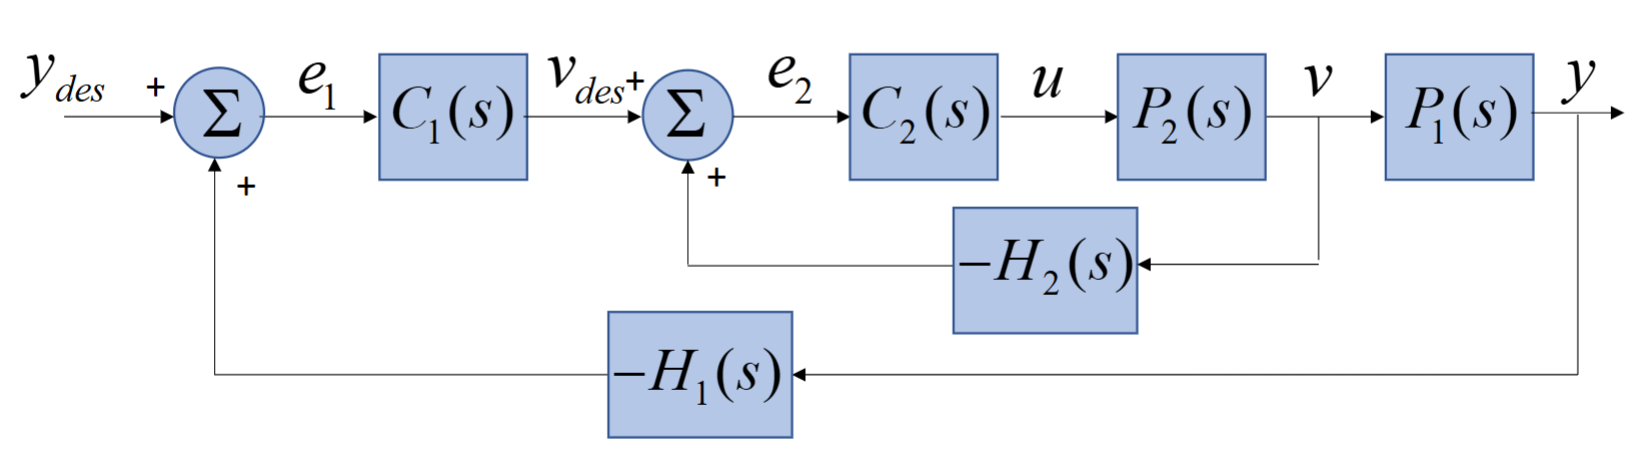
\includegraphics[width=0.8\linewidth]{Images/controls_blockexample1.png}
\end{center}

\textbf{Solution}. Observe that there are two closed loops: one outer loop, and one inner loop. These transfer functions are respectively given by: \[G_{fb,1} = P_1(s) P_2(s) C_2(s) C_1(s) (-H_1(s))= -P_1(s)P_2(s)C_2(s)C_1(s)H_1(s),\hspace{0.1in} G_{fb,2} = P_2(s) C_2(s) (-H_2(s)) = -P_2(s)C_2(s)H_2(s)\] There is only one forward path from $y_{des}$ to $y$ which overlaps both loops, namely the top path, which has a transfer function given by: \[G_{ff,1} = P_1(s) P_2(s) C_2(s) C_1(s)\] Applying Mason's rule gives the transfer function for the entire system: \begin{eqnarray*}
    G(s) &=& \frac{\sum_{i=1}^1 G_{ff,i}}{1 - \sum_{j=1}^2 G_{fb,j}}\\
    &=& \frac{P_1(s)P_2(s)C_2(s)C_1(s)}{1 - (-P_1(s)P_2(s)C_2(s)C_1(s)H_1(s)  - P_2(s)C_2(s)H_2(s))}\\
    &=& \boxed{\frac{P_1(s)P_2(s)C_2(s)C_1(s)}{1 + P_1(s)P_2(s)C_2(s)C_1(s)H_1(s) + P_2(s)C_2(s)H_2(s)}}
\end{eqnarray*}

Transfer functions provide a simple way to analyze complicated interconnected systems; however, the analysis is limited to linear, time-invariant systems, and they can be tedious to derive for high degree of freedom systems. An alternative method is to represent a system in \textit{state space}, which has the additional benefit in many engineering applications that future values are predictable from only the present values.

\begin{shaded}
    \textbf{State Space Representation}. A state space is a system of $n$ first-order differential equations of the following form: \[\begin{cases}\dot{\vec{x}} = f(\vec{x}, \vec{u})\\
    \vec{y} = g(\vec{x},\vec{u})\end{cases}\] where $\vec{x}$ is the \textit{state vector}, which is a collection of state variables. In the state-space representation, future values of the state variables depend \textit{only} on the present values of the state variables; i.e. both the present output $\vec{y}$ and the derivatives $\dot{\vec{x}}$ are functions of only the present values of the state $\vec{x}$.

    For \textit{linear} systems, the state-space representation is given by: \[\begin{cases}
        \dot{\vec{x}} = A\vec{x} + B \vec{u}\\
        y = C\vec{x} + D \vec{u}
    \end{cases}\] in which case the eigenvalues of $A$ give the roots of the characteristic polynomial (i.e. the roots of the denominator of a transfer function for the same system).

    All first-order differential equations can be represented in a block diagram solely through combinations of integrators (to eliminate derivatives), gains, and summation junctions. This can be accomplished by analyzing each equation in the state-space representation and relating present outputs to integrations and sums of others.
\end{shaded}

When applicable (i.e. for linear systems), there is a standard method for converting between the state space representation and the transfer function. In particular, consider a general linear time-invariant system of the form: \[y^{(n)} + a_{n-1}y^{(n-1)} + \cdots + a_1\dot y + a_0 y = b_mu^{(m)} + b_{m-1}u^{(m-1)} + \cdots + b_1 \dot u + b_0 u\] The transfer function representation is given by:

\[G(s) = \frac{b_m s^m + b_{m-1}s^{(m-1)} + \cdots + b_1 s + b_0}{s^n + a_{n-1}s^{(n-1)} + \cdots + b_1 s + b_0}\]

A state space representation for this system, known as \textit{controllable canonical form}, is given by:

\[\begin{bmatrix}
    \dot x_1\\
    \dot x_2\\
    \vdots\\
    \dot x_{n-1}\\
    \dot x_n
\end{bmatrix} = \underbrace{\begin{bmatrix}
    0 & 1 & 0 & \cdots & 0\\
    0 & 0 & 1 & \cdots & 0\\
    0 & 0 & 0 & \cdots & 0\\
    \vdots & \vdots & \vdots & \ddots & \vdots\\
    -a_0 & -a_1 & -a_2 & \cdots & -a_{n-1}    
\end{bmatrix}}_A\begin{bmatrix}
    x_1\\
    x_2\\
    \vdots\\
    x_{n-1}\\
    x_n
\end{bmatrix} + \underbrace{\begin{bmatrix}
    0\\
    0\\
    \vdots\\
    0\\
    1
\end{bmatrix}}_B u\] \[\vec{y} = \underbrace{\begin{bmatrix}
    b_0 & b_1 & \cdots & b_{n-2} & b_{n-1}
\end{bmatrix}}_C \vec{x}\] These representations are equivalent, and a simple mapping occurs by matching coefficients.

\subsection{Electromechanical Systems}

In a rigid body, the distance between any two points are fixed. The number of degrees of freedom for a system of rigid bodies is a sum of the rotational and translational degrees of freedom of each \textit{kinematically independent} rigid body in the system. Consider Newton's law in general form, relative to an inertial frame (i.e. a coordinate system which is not accelerating or rotating): \[\vec{F} = \frac{d}{dt}(m\vec{v})\] In this equation, $m(t)$ is a scalar, and both $\vec{F}$ and $\vec{v}$ are column vectors of size $3$. Euler's equation in general is of the form: \[\vec{M} =\frac{d}{dt}(I\vec{\omega})\] Note that $I$ is a $3\times 3$ matrix in general, and $\vec{\omega}$ and $\vec{M}$ are column vectors of size $3$. In the plane, there is only one rotational degree of freedom, so $I$ can be treated as a scalar and $M=I\omega$ a scalar equation.

\begin{framed}
\textbf{Newton-Euler Methods for Multiple Kinematically Constrained Bodies}. Consider a system of multiple kinematically constrained rigid bodies. Then, there is only one degree of freedom governing the total system. The general steps for deriving an equation of motion in this case are as follows: \begin{enumerate}
    \item[1.] Write $\vec{F}=m\vec{a}$ and/or $\vec{M}=I\vec{\alpha}$ for each rigid body.
    \item[2.] Write and substitute the kinematic constraints between each rigid body in terms of the desired variable.
    \item[3.] Rearrange for the desired motion variable; from here, integration (numerical or analytical) can be carried out.
\end{enumerate} This is known as the \textit{Newton-Euler method}, which involves force and moment balances. This process is applicable for any mechanical system and extends beyond planar mechanics, although it can become tedious due to the number of internal forces.
\end{framed}



An energy balance can achieve the same result, known as the \textit{Euler-Lagrange method}. It should be noted that, with multiple degree of freedom systems, energy methods can quickly become unworkable without more advanced techniques (i.e. the Lagrangian). In particular, an energy balance of even two compliantly constrained bodies may result in a single equation with two unknown position variables. The best approach is generally to solve a system of equations from balancing forces and moments. Regardless, the general process for single degree of freedom systems is provided.

\begin{framed}
\textbf{Euler-Lagrange Method for Multiple Kinematically Constrained Bodies}. Consider a system of multiple kinematically constrained rigid bodies (i.e. a system with one degree of freedom, which is critical to this case). The general steps for deriving an equation of motion with energy methods are as follows: \vspace{-1em}\begin{enumerate}
    \item[1.] Write the expressions for kinetic and potential energy for the entire system.
    \item[2.] Write the energy conservation equations: \[\frac{d}{dt} (KE + PE) = P_{in}-P_{out}\] where $P_{in}$ is the power into the system, and $P_{out}$ is the power out of the system.
    \item[3.] Substitute kinematic constraints for the desired variable and rearrange.
\end{enumerate}\vspace{-1em} The advantage of energy methods is that one does not need to solve for internal forces and constraints.
\end{framed}

Certain elements are especially common in mechanical systems; these are \textit{springs}, and \textit{dampers}. A \textit{spring} is a mechanical device which produces tensile or compressive force in response to elongation or contraction respectively. A \textit{linear spring} of stiffness $k$ produces force $F_s$ which is linearly proportional to elongation $s$: \[F_s = ks\] A linear \textit{torsional spring} produces a restoring torque which is directly proportional to relative angular displacement. For a torsional spring with constant $k_T$ and relative angular displacement $\phi$, the restoring torque is given by: \[T_s = k_T\phi\] In either case, the spring stores potential energy.

A \textit{damper} is a mechanical device which produces a tensile or compressive force in response to the rate of elongation. A \textit{linear damper} with damping coefficient $c$ produces force $F_d$ which is linearly proportional to the elongation rate: \[F_d = c\frac{ds}{dt}=c\dot s\] Similarly, for a torsional damper with constant $c_T$, the restoring torque is given by: \[T_d = c_T \frac{d\phi}{dt} = c_T\dot\phi\] Dampers dissipate energy, so they contribute to $P_{out}$, generally in the form of friction.

The analysis of electromechanical systems can be reduced to analysis of motors and/or generators. This requires an analysis of circuits containing voltage sources, resistors, capacitors, and inductors. Two conservation laws govern all electrical systems generally. 

Kirchoff's Current Law gives a conservation of charge. In particular, the net current $I_{in}$ into a node must equal the net current $I_{out}$ leaving that node. \[I_{in} = I_{out} \tag{Kirchoff's Current Law}\] Kirchoff's Voltage Law gives a conservation of energy. In particular, the potential difference, or voltage, around any closed loop must sum to $0$. Then, for a closed loop with $k$ voltages $V_k$: \[\sum_{k=1}^n V_k = 0\tag{Kirchoff's Voltage Law}\]

A \textit{resistor} is a device which produces a voltage drop $\Delta V$ that is proportional to current $I$. That is, an (ohmic) resistor with resistance $R$ produces a voltage drop given by: \[\Delta V=IR\tag{Ohm's Law}\] Resistors dissipate energy from a circuit in the form of heat. A \textit{capacitor} is a device which produces a voltage drop that is proportional to stored charge. That is, \[q = \int_0^t I d\overline{t}\] More usefully, for a capacitor with capacitance $C$, this can be written to relate voltage and current: \[\Delta V = \int_0^t \frac{1}{C} I d\overline{t}\] which is the constitutive relation for capacitors. Equivalently, this yields the following differential equation for voltage in a capacitor: \[\dot V_C = \frac{1}{C}I\] An \textit{inductor} is an electrical device which produces a voltage drop that is proportional to the change in current, $\dot I$. That is, \[V_L = L\frac{dI}{dt}\] Both inductors and capacitors store electrical energy.

\begin{framed}
    \textbf{General Process for Circuit Analysis}. In general, only two things are known about a circuit: Kirchoff's laws, and constitutive relations for circuit components. Therefore, the general steps for analyzing a circuit are as follows:
    \vspace{-1em}
    \begin{enumerate}
        \item[1.] Write Kirchoff's laws for the circuit; this may involve Kirchoff's voltage law for some or all of the loops, and/or Kirchoff's current law for some of the nodes.
        \item[2.] Write constitutive relations for relevant components; this involves Ohm's law for resistors, and other relationships for other components (i.e. for inductors and capacitors).
    \end{enumerate}
\end{framed}

The \textit{impedance} is a generalization of resistance; by definition, $Z(s)$ is the ratio of voltage to current in the Laplace domain, i.e. it is defined as a transfer function: \[Z(s) = \frac{V(s)}{I(s)}\] Note that the impedance across a resistor of resistance $R$ is simply $R$. Impedance of an arbitrary portion of a circuit can be found by superposition of impedance for each components, which is found by taking a Laplace transform of the constitutive relationships. Impedences behave as resistors, obeying the same properties for addition in series and parallel as Ohmic resistors.

In general, electrical power is given by \[P=IV\] Substituting constitutive relationships, this allows one to calculate the power dissipated or stored by the components. Using this fact, the maximum power transfer across a resistor can be calculated.

\begin{shaded}
    \textbf{Maximum Power Transfer in a Resistive Load}. Consider a system consisting of a source voltage input $V_s$, a system resistance $R_s$, and a load resistance $R_L$ in series, across which there is a voltage drop $V_0$. Applying Kirchoff's laws: \[V_0 = \frac{R_L}{R_s+R_L} V_S\] and \[I = \frac{V_s}{R_s + R_L}\] The power is given by: \[P - V_0 I = \frac{R_L}{(R_s+R_L)^2} V_s^2\] Differentiation with respect to $R_L$ and considering when the numerator equals $0$ gives the optimal load resistance $R_L^*$ for power transfer: \[0 = V_s^2 (R_s^2 - R_L^2) \implies \boxed{R_L^* = R_s}\] This is the \textbf{impedance matching principle}; that is, the impedance of the output should be designed to match the impedance inherent to the circuit.
\end{shaded}

Energy methods are possible with circuits, but they are not generally necessary; the primary motivator for energy methods in mechanical systems was to avoid calculating internal forces, which are not present in electrical circuits. For this reason, considering Kirchoff's laws with the constitutive relationships is generally the more straightforward approach.
\vspace{1em}

\begin{framed}
An \textbf{electromechanical system} is comprised of an electrical circuit, a mechanical system, and \textit{coupling equations} which relate the circuit model to the mechanical model. 

Every mechanical system attached to an electrical system can be modeled as either a motor or a generator, where a generator is just a motor operating in reversed current direction. In general, the coupling equations will take a similar form: \[\begin{cases}
    V = K_b \omega\\
    T = K_T I
\end{cases}\] where $T$ is the motor or generator torque, $\omega$ is the motor or generator speed, $V$ is the voltage drop across the motor or generator, and $I$ is the current through the motor or generator. In a motor, $K_b$ is a proportionality between the \textit{back-emf} and motor speed; in a generator, this is typically denoted $K_g$ instead.
\end{framed}

\subsection{Time and Frequency Analysis}

\textbf{Time-domain analysis} is concerned with predicting outputs in terms of an observed system input and known system components, or identifying system parameters from observed system response to known inputs. Attention will be restricted to first- and second-order linear time-invariant systems, with forcing functions taking only the form of impulse, steps, or ramps.

\begin{framed}
    \textbf{First-Order System Response}. Consider systems of the form $\dot x + a x = u(t)$ for some forcing function $t$. Analysis will be carried out for impulse and step functions $u(t)$.

    \textit{Impulse Response}. Consider a system $\dot x + a x = b\delta(t)$ with an initial condition at $x(0^-)$, i.e. immediately before the impulse. Taking Laplace transforms, this gives: \[sX(s) - x(0^-) + a X(s) = b \implies X(s) = \frac{x(0^-) + b}{s+a} \implies \boxed{x(t) = x(0^-) e^{-at} + be^{-at}}\] where the time constant for decay is given by $\tau = \frac{1}{a}$, and the steady-state value is $0$.

    \textit{Step Response}. A system with step of size $b$ behaves identically to a system forced by a constant input $b$ for $t\geq 0$, and this analysis has been previously carried out. In this case, the method of characteristics gives a solution of the form: \[\boxed{x(t) = \left(x(0) - \frac{b}{a}\right) e^{-at} + \frac{b}{a}}\] where the time constant is again $\tau = \frac{1}{a}$, and the steady-state value is now $\frac{b}{a}$. Note that the \textit{settling time}, where $x(t)$ reaches $98\%$ of its steady-state value, is at $t=4\tau$, and that this steady state value is exactly the DC gain of the system multiplied by the input signal (i.e. the step of size $b$).
\end{framed}

Similar analysis extends to second-order systems, with the important caveat that response to jumps in input are \textit{not} instantaneous for these systems; in particular, an impulse causes an instantaneous jump in \textit{velocity}, rather than position. Furthermore, second-order systems may experience oscillations and overshoot past the steady-state value, and therefore additional information is typically needed to fully describe the motion of a second-order system; namely, a second-order system can be put into the form \[\ddot x + 2\zeta\omega_n \dot x + \omega_n^2 x = f(t)\] The damped natural frequency $\omega_d$, which is the frequency of oscillations observed in the system, is related to these parameters by \[\omega_d = \omega_n \sqrt{1-\zeta^2}\] Note that for $\zeta=0$, i.e. undamped motion, the frequency of oscillations is exactly the natural frequency. The time constant for such a system is given by: \[\tau = \frac{1}{\zeta\omega_n}\] Relationships between these quantities, as well as the steady state behavior and time constant as found in first-order system analysis, is enough to describe the dynamics of a system (including the period and the system parameters). 

\begin{shaded}
\textbf{Parameter estimation}. A process to estimate a system's parameters can be carried out whenever a system's input and response is known in time. Consider a first-order system with a transfer function of the following form: \[G(s) = \frac{b}{s+a}\] The ratio $b/a$ can be found from the DC gain: \[G(0) = \frac{b}{a} \implies x_{steady} = u \frac{b}{a} \implies \frac{b}{a} = \frac{x_{steady}}{u}\] However, the pole of $G(s)$ is at \[ s + a = 0 \implies s = -a \implies \tau = \frac{1}{a}\] It follows that the time $t$ such that $x(t) = 0.63\cdot x_{steady}$ has the property that $t=\tau = \frac{1}{a}$. From these two constraints, both $a$ and $b$ can be found. 

For data which is noisy, a least-squares estimate can be used instead. For sake of illustration, consider the same first-order system, which has an expected solution form \[x(t) = x(0) e^{-\frac{1}{\tau} t}\] Taking logarithms of both sides: \begin{eqnarray*}
    \ln[x(t)] &=& \ln \left[[x(0)e^{-\frac{1}{\tau} t}\right]\\
    &=& \ln [x(0)] + \ln e^{-\frac{1}{\tau} t}\\
    &=& \ln [x(0)] - \frac{1}{\tau} t
\end{eqnarray*} That is, there is a linear relationship \[\ln\big[ x(t)\big] = \ln \big[ x(0)\big] - \frac{1}{\tau} t\] where a trendline through data is expected to produce an intercept at $\ln \big[ x(0)\big]$ and a slope $-\frac{1}{\tau}$.

It should be noted that, near steady-state, errors are amplified by the logarithm because the difference $x_{ss} - x(t)$ between the actual value and the steady-state value becomes very small, causing the logarithm of the error to become very large; therefore, even with constant error, the logarithm of the error increases with time. Intuitively, this means that the system parameters are most obvious when the transients are strongest. For this reason, it is often beneficial to only consider transient data for parameter estimation.
\end{shaded}

\newpage
\textbf{Frequency-domain analysis} is concerned with persistent, periodic inputs. Since well-behaved periodic inputs can be written as their Fourier series, and therefore as a sum of sine waves of different frequencies, it suffices to consider periodic inputs of the form $u(t) = A\sin(\omega t)$. For a stable, linear time-invariant system with this input profile, the \textit{steady-state output} $x_{ss}(t)$ of the system will take the form $x_{ss}(t) = B\sin(\omega t + \phi)$. Analysis of this transfer function shows: \begin{eqnarray*}
    Y(s) &=& G(s)U(s)\\
    &=& G(s) \underbrace{A\frac{\omega}{s^2+\omega^2}}_{A\sin(\omega t)}\\
    &=& A\left[\frac{N(s)}{(s-p_1)\cdots (s-p_n)}\right] \cdot \frac{\omega}{(s+i\omega)(s-i\omega)} \hspace{0.2in}\text{for some numerator }N(s)\text{ and poles }p_1,\dots,p_n\\
    &=& A \left[\frac{a_1}{s-p_1} + \cdots + \frac{a_n}{s-p_n} + \frac{b}{s+i\omega} + \frac{\overline{b}}{s-i\omega}\right] \hspace{0.2in} \text{by PFD for some }a_1,\cdots,a_n,b,\overline{b}\\
\end{eqnarray*} Inverse Laplace transformation gives: \[y(t) = \underbrace{a_1 e^{p_1 t}+ \cdots + a_ne^{p_nt}}_\text{transients} + \underbrace{be^{i\omega t} + \overline{b} e^{-i\omega t}}_\text{steady state}\] By some rearrangement and applying Euler's formula, it can be shown that \[y(t) = A|G(i\omega)|\sin(\omega t + \phi)\] where $|G(i\omega)|$ is the magnitude of the transfer function evaluated at $s=i\omega$ and $\phi$ is the angle of the vector $G(i\omega)$. The general method for evaluating steady-state outputs is to evaluate the magnitude and argument of $G(i\omega)$, which yields all the necessary information to describe the steady-state output.



\begin{shaded}
    \textbf{Properties of Bode Plots}. Given a stable linear time-invariant system, a \textbf{Bode plot} separately graphs two system properties, namely the system gain, given by $G:=B/A$, and the phase shift, $\phi$, as functions of $\omega$. Bode plots typically measure system gain in decibels, where the gain expressed in decibels is given by $|M(i\omega)|_{dB}:= 20\log_{10}|G(i\omega)|$. The slope of a Bode plot is often measured in decibels per decade, where a decade corresponds to a $10$-fold increase in frequency.
    
    Zeroes and poles have distinct behavior on a Bode plot. In particular, zeroes and poles have an effect on the slope and phase shift, with these changes centered around the \textit{corner frequency}, or \textit{cutoff frequency}, which is the value $\omega_c$ associated with each zero or pole.
    \vspace{-1em}
    \begin{enumerate}
        \item[] \textbf{First Order Zeroes} contribute a slope of $+20\text{dB/dec}$ to the gain plot, and a phase shift of $+90^\circ$ phase lead.
        \item[] \textbf{Second Order Zeroes} contribute a slope of $+40 \text{dB/dec}$ to the gain plot, and a phase shift of $+180^\circ$ phase lead.
        \item[] \textbf{First Order Poles} contribute a slope of $-20\text{dB/dec}$ to the gain plot, and a phase shift of $-90^\circ$ phase lag.
        \item[] \textbf{Second Order Poles} contribute a slope of $-40\text{dB/dec}$ to the gain plot, and a phase shift of $-180^\circ$ of phase lag.
    \end{enumerate}
    \vspace{-1em}
    All polynomials can be factored into either first- or second-order real factors, so this is an exhaustive list of cases. Two facts should be noted:
    \vspace{-1em}
    \begin{enumerate}
        \item[1.] At a particular $\omega_c$, the phase shift reaches its midpoint; for example, at $\omega_c$ corresponding to a first order zero, the Bode phase plot shows a $+45^\circ$ phase lead at $\omega_c$.
        \item[2.] For systems with a second-order pole or zero, a \textit{resonant peak} may occur if the system has a damping ratio in the range $\zeta\in [0,\sqrt{2}/2]$. In this case, there is a distinct resonant frequency $\omega_r$ at which a resonant peak is visible at a multiple $M_r$ of the DC gain; these quantities can be found by: \[\omega_r = \omega_n\sqrt{1-2\zeta^2},\hspace{0.5in} M_r = \frac{\text{Peak Gain}}{\text{DC Gain}} = \frac{1}{2\zeta\sqrt{1-\zeta^2}}\] There is also a resonant phase shift $\phi_r$, which can be found by \[\phi_r = -\arctan\left(\frac{\sqrt{1-2\zeta^2}}{\zeta}\right)\]
    \end{enumerate}
\end{shaded}

\textbf{Example}. Consider a system with transfer function \[G(s) = \frac{s+100}{s^2+s+10}\] The quadratic formula shows that $G$ has a pole at $s=-\frac{1}{2} \pm \frac{\sqrt{39}}{2}i$, and therefore $\omega_{c_1} = \left|-\frac{1}{2} \pm \frac{\sqrt{39}}{2} i\right| \approx 3.2\ \text{rad/s}$. This is a second-order pole, so it contributes phase lag of $-180^\circ$ and (with a phase lag of $-90^\circ$ occurring at $\omega_{c_1}$), and a slope of $-40\text{ dB/dec}$. The damping ratio for this system is \[2\zeta\omega_n = 1 \implies \zeta = \frac{1}{2\sqrt{10}} \approx 0.16\] Therefore, there is a resonant frequency and a resonant peak, and these values are approximately: \[\omega_r \approx 3.1 \text{ rad/sec},\hspace{0.5in}M_r \approx 3.2\] which corresponds to a $10\text{ dB}$ increase above the low-frequency gain. 

$G$ also has a zero at $s=-100$, and therefore $\omega_{c_2} = 100\text{ rad/sec}$. This corresponds a contribution of $+90^\circ$ phase lead, with a $+45^\circ$ contribution at $\omega_{c_2}$, as well as a contribution of $+20\text{ dB/dec}$.

Together, this corresponds to the following Bode plot:

\begin{center}
    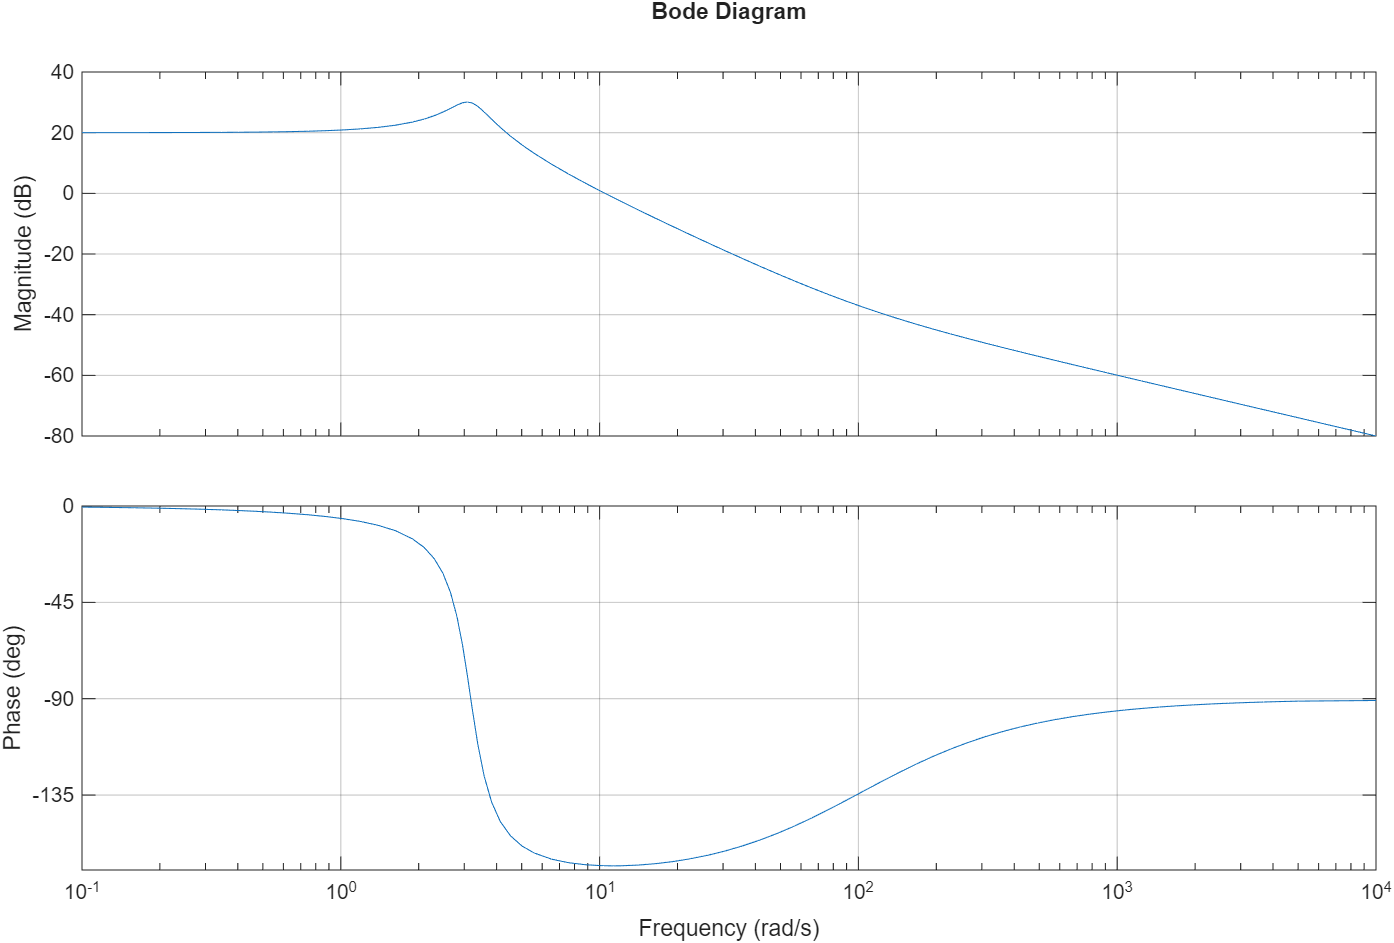
\includegraphics[scale=0.3]{Images/controls_bode.png}
\end{center}

\begin{shaded}
    \textbf{Overshoot and Undershoot}. The \textit{numerator dynamics}, given by the zeros of the system's transfer function, determine whether a system will overshoot or undershoot.

    If a zero is a \textbf{minimum phase zero}, i.e. the zero is in the left-half of the complex plane and contributes a phase lead, it will contribute \textit{overshoot}, where the response will initially exceed a steady input. If a zero is a \textbf{non-minimum phase zero}, i.e. the zero is in the right-half of the complex plane and contributes a phase lag, it will contribute \textit{undershoot}, and the response will initially move away from a steady input.
\end{shaded}

\newpage\subsection{Control Systems}

A control system \textit{in general} involves four blocks: a controller, an actuator, a plant, and a feedback loop with a sensor. These control systems also take a setpoint (desired output) as an input signal, as well as disturbance signals. In practice, many control systems utilize actuators and sensors which respond rapidly in comparison to the mechanical components, i.e. the plant. Because the time constants associated with the sensor and actuator are small, these blocks can often be neglected from the system dynamics (replaced with a unit gain). This results in a system with two blocks: a controller, which produces a control signal based on an error input signal, and a plant.

Below is a full feedback loop with sensor dynamics $H(s)$, controller dynamics $G_c(s)$, actuator dynamics $G_a(s)$, and plant dynamics $G_p(s)$. With the above simplifications, it is often reasonable to set $G_a(s)=H(s)=1$, in which case these blocks could be excluded from the diagram.

\begin{center}
    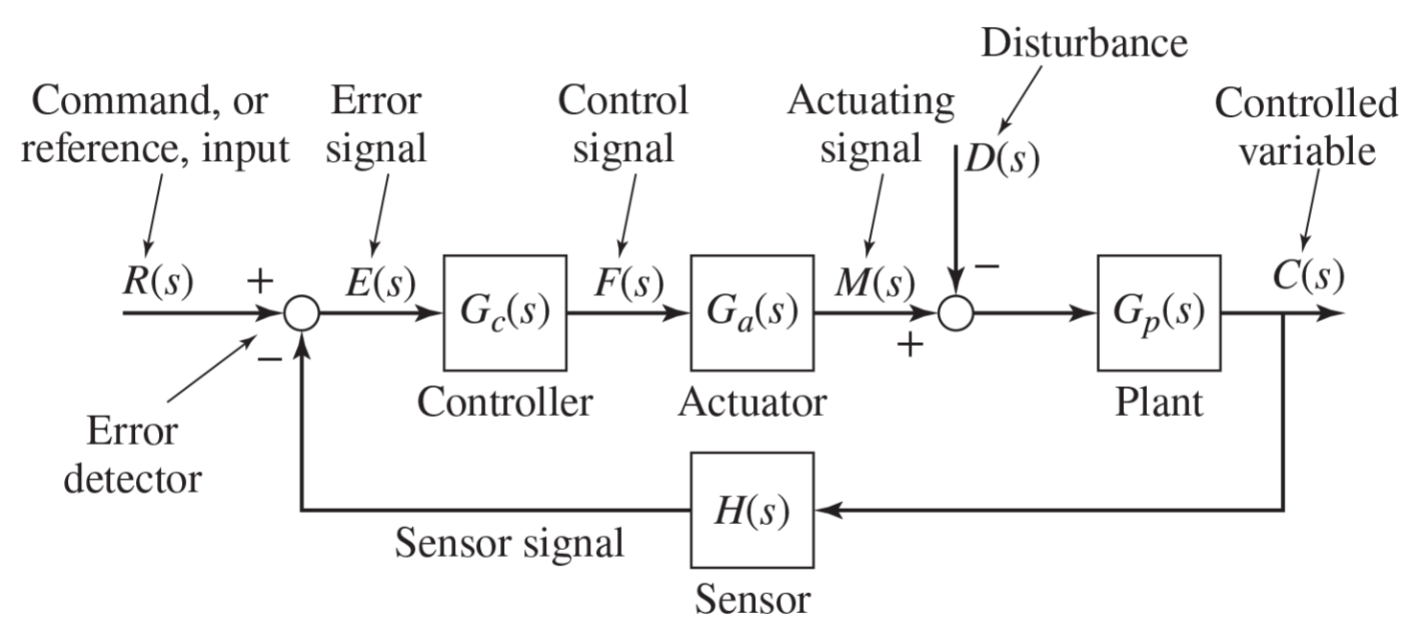
\includegraphics[scale=0.325]{Images/controls_sensorsystem.png}
\end{center}

A discussion of control laws will tend to yield higher-order systems, where the stability criteria are more complicated than for second order systems alone. A brief discussion on these conditions will be provided:

\begin{shaded}
    \textbf{Routh-Hurwitz Stability Condition}. The Routh-Hurwitz condition gives algebraic constraints for when a polynomial has roots with negative real parts. The Routh-Hurwitz condition can be applied to the denominator of the closed-loop transfer function to determine the stability of a system. This condition is necessary because when coupled with the plant dynamics, many closed-loop systems have higher-order poles than second order, where the stability condition is simple. These rules generally set practical limits on the gains which can be chosen in PID control.

    For this discussion, assume that for an $m$-order system, the highest-order coefficient $a_m$ is positive. If this is not the case, divide through by $-1$ and apply the conditions.

    \begin{enumerate}
        \item[] \textbf{Second-Order}: A system with dynamics $a_2s^2 + a_1 s + a_0 = 0$ is stable $\iff$ $a_0,a_1,a_2>0$.
        \item[] \textbf{Third-Order}: A system with dynamics $a_3s^3 + a_2s^2 + a_1s + a_0 = 0$ is stable $\iff$ $a_0,a_1,a_2,a_3>0$ and $a_2a_1 > a_3a_0$.
        \item[] \textbf{Fourth-Order}: A system with dynamics $a_4s^4 + a_3s^3 + a_2s^2 + a_1s + a_0$ is stable $\iff$ $a_0,a_1,a_2,a_3,a_4>0$, $a_2a_3 > a_1a_4$, and $a_1(a_2a_3 - a_1a_4) - a_0a_3^2 > 0$.
    \end{enumerate}
\end{shaded}
\vspace{-1.5em}
In the following discussion, let $u(t)$ be the control signal (output of the controller), and $e(t)$ be the error signal (input to the controller). Various control schemes which feed into the plant will now be analyzed.

\textbf{On-Off Control}. An on-off control system specifies a value (either ON or OFF) according to the present error; that is, the controller produces a control signal $u(t)$ of the form: \[u(t) = \begin{cases}
    u_{max},\ & e(t)<0\\
    0,\ & e(t)=0\\
    -u_{max},\ & e(t)>0
\end{cases}\] Note that this is a static, nonlinear control law. A hysteresis band is often used to prevent chattering about the setpoint.


\textbf{PID Control}. A proportional-plus-integral-plus-derivative controller, or PID controller, produces a control signal of the form \[u(t) = K_p e(t) + \int_0^t K_i e(\bar{t}) d\bar{t} + K_d \frac{de}{dt}\] The transfer function from the error $E(s)$ to the control signal $U(s)$ can be derived from rearrangement: \[\frac{U(s)}{E(s)} = \frac{K_ds^2 + K_ps + K_i}{s}\tag{PID Control}\] Interestingly, this shows that this control law has a \textit{non-causal} relationship, since the numerator polynomial has greater degree than the denominator polynomial; the future values in practice are approximated by numerical differentiation schemes, which makes implementation possible.

Different control schemes can be implemented by simply setting particular gains to $0$. For example, for $K_d=K_i=0$, the control law reduces to \textit{position control}, with a control law given by \[\frac{U(s)}{E(s)} = K_p\tag{P-Control}\] This control scheme produces a plant input $u$ in direct proportion to the error between the current state and a setpoint. note that if a constant, non-zero control signal is necessary to maintain the setpoint, proportional control alone is \textit{not capable} of maintaining the setpoint. This motivates the introduction of an integral term.

For $K_d=0$, the control law reduces to \textit{position-integral control}, or PI control, with a control law given by \[\frac{U(s)}{E(s)} = \frac{K_p s + K_i}{s} \tag{PI-Control}\] Note that this is not, on its own, stable in the bounded input-bounded output sense. However, if $K_p$ and $K_i$ are chosen in a sensible way to guarantee stability, the system \textit{will} have perfect steady-state tracking. Additionally, windup on the integral term can produce large overshoot and long settling times if $K_i$ is too large.

For $K_i = 0$, the control law reduces to \textit{position-derivative control}, or PD control, with a control law given by \[\frac{U(s)}{E(s)} = K_p + K_d s\tag{PD-Control}\] It is clear that the derivative term introduces non-causality into the control law; i.e. the derivative term anticipates future values of the error by providing desired signal proportional to the rate of change of the error. The derivative term can be used to increase damping, although a drawback is that derivative gains can amplify errors.

PID control has the benefit that it improves transient response through the derivative control while decreasing (or eliminating) steady-state error through the integral control. However, the parameters must be selected carefully so that a system is stable.

\begin{framed}
    \textbf{Selection of Gains}. The following discussion gives some general guidance for selecting reasonable gains for PID control.

    It should be noted that gains have dimensions; for example, if $u(t)$ is a commanded speed in m/s and $e(t)$ is a position error in meters, then the proportional gain $K_p$ must have units $1/s$. $K_p$ should then be chosen so that $K_p e(t)$ is a sensible number for an expected error $e(t)$. For example, if the system should command a speed of $4$ m/s in response to $1$ m of error, then $K_p\approx 4$ is a reasonable initial choice of gain.

    $K_i$ and $K_d$ can be chosen in terms of $K_p$. In particular, suppose $\tau_{cl}$ is the desired closed-loop time constant of the system. Dimensional analysis shows that the units of $K_i$ are $[K_i] = [K_p]/s$, and the units of $K_d$ are $[K_d] = [K_p]\cdot s$; that is, the $dt$ must "cancel" with a unit $1/s$ in $K_i$, and the "$1/dt$" must "cancel" with a unit $s$ (where $s$ is seconds, but could be any other time unit as is sensible for the system). Therefore, reasonable choices for $K_i$ and $K_d$ are, respectively: \[K_i \approx \frac{K_p}{\tau_{cl}},\hspace{1.5in} K_d \approx K_p \tau_{cl}\] These values do not always work, but these are reasonable guesses which can be tuned as necessary. Note that $K_p$, $K_i$, and $K_d$ must also be chosen such that the system is stable.

    \textbf{Example}. Consider a system with plant dynamics \[G(s) = \frac{b_0}{s^2+a_1 s + a_0}\] Select $K_i$, $K_p$, and $K_d$ such that the system has the following properties: \vspace{-1em}\begin{enumerate}
        \item[(i)] There is no steady-state error for a unit step input.
        \item[(ii)] Settling time is $3$ seconds.
        \item[(iii)] The system is overdamped.
    \end{enumerate}\vspace{-1em}
    \textbf{Solution}. Note that PID control has a general form: \[C(s) = \frac{K_ds^2+K_p s + K_i}{s}\] and Mason's rule gives: \begin{eqnarray*}
        \frac{X(s)}{U(s)} &=& \frac{G(s)C(s)}{1+G(s)C(s)}\\
        &=& \frac{\frac{b_0}{s^2+a_1s+a_0}\cdot \frac{K_ds^2+K_ps+K_i}{s}}{1+\frac{b_0}{s^2+a_1s+a_0}\cdot \frac{K_ds^2+K_ps+K_i}{s}}\\
        &=& \frac{b_0(K_ds^2+K_ps+K_i)}{s(s^2+a_1s+a_0) + b_0(K_ds^2+K_ps+K_i)}\\
        &=& \frac{b_0K_ds^2+b_0K_ps+b_0K_i}{s^3+(a_1+b_0K_d)s^2+(a_0+b_0K_p)s+b_0K_i}
    \end{eqnarray*}
    If requirements (ii) and (iii) are met, requirement (i) will automatically be met. In particular, for a system to have time constants or be overdamped, it must be stable. Therefore, any $K_i\neq 0$ will suffice as long as (ii) and (iii) are met.

    These requirements can be met by matching the denominator to a desired polynomial. A settling time of $3$ seconds is desired. Recall that settling time is given by $t_s \approx 4\tau$. Therefore, $\tau \approx 3/4$ is required, meaning one pole of the transfer function must have real part $\sigma = 4/3$. For overdamping, all poles must lie on the negative real axis. To ensure a settling time of $3$ seconds, these poles must respond much faster than $\tau$ so that $\tau$ remains the dominant time constant, i.e. these poles must be at least larger than $5\tau$. One choice which satisfies this is $s=10$. With these choices, a desired denominator polynomial satisfying this is given by: \[\operatorname{Den}_{des}(s) = (s+4/3)(s+10)^2\] Setting this equal to the actual denominator polynomial: \begin{eqnarray*}
        (s+4/3)(s+10)^2 &\equiv& s^3+(a_1+b_0K_d)s^2 + (a_0+b_0K_p)s + b_0K_i\\
        \implies s^3+\frac{64}{3}s^2+\frac{380}{3}s+\frac{400}{3} &=& s^3+(a_1+b_0K_d)s^2+(a_0+b_0K_p)s+b_0K_i
    \end{eqnarray*} Setting common factors equal, \[\begin{cases}
        64/3 = a_1+b_0K_d &\implies K_d = \frac{64/3 - a_1}{b_0}\\
        380/3 = a_0+b_0K_p &\implies K_p = \frac{380/3 - a_0}{b_0}\\
        400/3 = b_0K_i &\implies K_i = 400/(3b_0)
    \end{cases}\]
\end{framed}

\textbf{Combined Feedforward-Feedback Control}. Many control structures leverage both a feedforward loop, with transfer function $C_{ff}(s)$, and a feedback loop, with transfer function $C_{fb}(s)$. Given plant dynamics $P(s)$, Mason's rule gives a system transfer function of: \[\frac{Y(s)}{U(s)} = \frac{P(s)C_{ff}(s) + P(s)C_{fb}(s)}{1 + P(s) C_{fb}(s)}\] Note that, as long as the feedforward loop alone is stable, the feedforward component will have no effect on system stability. This structure has the substantial benefit that the system may respond faster than with feedback control alone while maintaining the flexibility of feedback control.

\textbf{Inner Loop/Outer Loop Control}. Many control structures leverage an inner loop $C_2(s)P_2(s)$ which rejects disturbances, alongside an outer loop $C_1(s)C_2(s)P_1(s)P_2(s)$ which tracks the setpoint. The transfer function for such a control scheme is given by: \[\frac{Y(s)}{U(s)} = \frac{P_1(s)P_2(s)C_2(s)C_1(s)}{1+P_2(s)C_2(s) + P_1(s)P_2(s)C_2(s)C_1(s)}\] This scheme is frequently used because it decouples disturbance and setpoint tracking, allowing these tasks to be carried out separately.